% Drawing 33/09-3 -- folder 33, batch 09, archive page 175 (PDF page 176).
% Transcription: deux axes, le long de l'axe horizontal un segment de $0$ à $2d$ marqué de points ; puis un triangle sous une droite de pente $-1$, strié de traits horizontaux, l'abscisse $2d$ marquée.
% Kind: axes with a graduated segment; hatched triangle under a line of slope -1. Method 2 (schematic redraw from the facsimile). Status: ok.
% Notes: Above: two axes crossing at a heavy point; along the horizontal one, an open point, a small point (the stretch after it doubled in pencil), and an angle mark at its end over the label 2d; a small open point on the vertical axis just above the origin. Below: axes (the vertical slightly slanted, the origin computed as their meeting point), a thin line of slope about -1, a heavy edge under it from the first step down to the horizontal axis at 2d (heavy point), a staircase of three vertical steps joined by short horizontals, and six horizontal hatching strokes from the vertical axis, each ending on the staircase where it does on the page (the third ends short, at the heavy edge); points on the heavy edge, three small points on the horizontal axis under the steps, a point on the vertical axis. Still differs: the heavy edge is a polyline through the points he marked, his stroke is smoother. Redrawn 2026-11-09 (issue 128): to check again. 2026-11-13, Claude Opus 5.5, overlay check (issue 147): the lower figure re-read on a millimetre grid of the scan rendered at 350 dpi in colour (21 px a unit); not compiled (no TeX engine in the session), the TikZ was rasterised by a script and laid over the crop. Redrawn as on the page: the staircase is three separate vertical steps (at about 62, 71 and 79), not a polyline with horizontal treads (the treads were drawn twice, over the hatching strokes); the heavy edge is a short heavy stroke along the thin line at the top, then a heavy stroke down through the marked points, dotted for a short stretch, down to the axis at 2d, doubled at its foot; of the six hatching strokes the third is two strokes (a heavy one reaching the thin line, a lighter one under it stopping short), the fifth reaches the third step; the points re-read (seven on the heavy edge and the steps, five on the horizontal axis, one on the vertical axis) and a speck beside the dotted stretch; the label 2d moved 2 units right onto its ink. The upper figure lies on its ink within about 1 unit and is unchanged. Everything now lies on its ink within about 1 unit.
% Coordinates: 1 unit = 1 mm = 1/100 of the crop width (bbox in page fractions: [0.07, 0.45, 0.35, 0.68]).
% Redrawn by Claude (claude-opus-5-5), issue #73, 2026-11-09; not checked by a human; not compiled (no TeX in the session).
% Rights: reproduces part of the work -- behind RENDER_TRANSCRIPTS, never published by itself.
\documentclass[tikz,border=3pt]{standalone}
\usepackage{amsmath,amssymb}
\usetikzlibrary{patterns,arrows.meta}
\tikzset{pencil/.style={black!45}, struck/.style={black!35}, mark/.style={circle,draw,inner sep=1.3pt}, pt/.style={circle,fill,inner sep=0.9pt}, opt/.style={circle,draw,fill=white,inner sep=1.1pt}}
\begin{document}
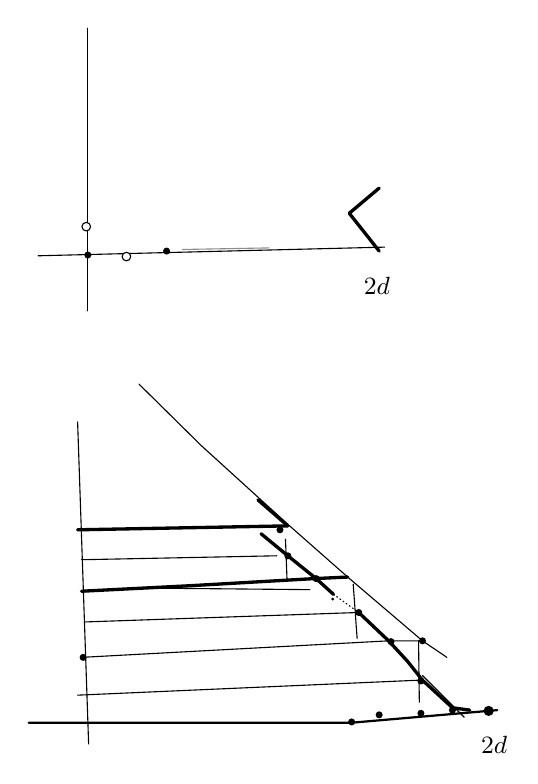
\begin{tikzpicture}[x=1mm,y=1mm,line cap=round,line join=round,font=\scriptsize]
\draw (37,-7) -- (37,-42.9);
\draw (30.7,-35.9) -- (74.7,-34.8);
\node[pt] at (37,-35.8) {};
\node[opt] at (36.8,-32.2) {};
\node[opt] at (41.9,-36) {};
\node[pt] at (47,-35.3) {};
\draw[pencil] (49,-35.1) -- (60,-34.9);
\draw[very thick] (74,-27.3) -- (70.2,-30.5) -- (74,-35.3);
\node[inner sep=1pt] at (73.7,-39.7) {\small $2d$};
\draw (35.7,-57) -- (37.1,-97.9);
\draw[thick] (29.5,-95.2) -- (70.5,-95.2) -- (89,-93.6);
% the thin line of slope about -1
\draw (43.5,-52.2) -- (51.4,-60) -- (62.4,-70) -- (70,-76.7) -- (79.5,-84.8) -- (82.6,-86.9);
% the heavy edge under it
\draw[very thick] (58.6,-66.9) -- (62.4,-70.2);
\draw[very thick] (59,-71.2) -- (62.4,-74) -- (66,-76.9) -- (68.2,-78.9);
\draw[densely dotted] (68.2,-78.9) -- (71.4,-81.2);
\draw[very thick] (71.4,-81.2) -- (75.2,-84.8) -- (77.6,-87.4) -- (79.5,-89.8) -- (83.3,-93.3) -- (85.5,-93.6);
\draw (79.5,-89.2) -- (84.8,-94.5);
% three vertical steps
\draw (62.1,-71.9) -- (62.3,-77.1);
\draw (70.7,-77.6) -- (71.2,-84.5);
\draw (79,-84.8) -- (79.1,-92.6);
% horizontal hatching from the vertical axis
\draw[very thick] (35.7,-70.7) -- (62.4,-70.2);
\draw (36.2,-74.5) -- (61,-74);
\draw[very thick] (36.2,-78.5) -- (50,-77.8) -- (65.7,-76.9) -- (70,-76.7);
\draw (44.3,-78.1) -- (65.2,-78.3);
\draw (36.7,-82.4) -- (71.4,-81.2);
\draw (36.2,-86.9) -- (75.2,-84.8) -- (79.5,-84.8);
\draw (35.7,-91.7) -- (79,-89.8);
% points
\node[pt] at (61.4,-70.7) {};
\node[pt] at (62.4,-74) {};
\node[pt] at (66,-76.9) {};
\node[pt] at (71.4,-81.2) {};
\node[pt] at (75.5,-84.9) {};
\node[pt] at (79.5,-84.8) {};
\node[pt] at (79.3,-89.9) {};
\node[pt] at (70.5,-95.1) {};
\node[pt] at (74,-94.2) {};
\node[pt] at (79.3,-94) {};
\node[pt] at (83.3,-93.6) {};
\node[pt,inner sep=1.3pt] at (87.9,-93.7) {};
\node[pt] at (36.4,-86.9) {};
\fill (68.1,-79.5) circle[radius=0.2];
\node[inner sep=1pt] at (88.6,-98) {\small $2d$};
\end{tikzpicture}
\end{document}
